\chapter{Indexation par termes-clés en domaine de spécialité}
\label{chap:main-domain_specific_keyphrase_annotation}
  \chaptercite{
    [\dots] the essential challenge of keyphrase extraction is the vocabulary
    gap between documents and keyphrases.
  }{
    \newcite{liu2011vocabularygap}
  }

  %-----------------------------------------------------------------------------

  \section{Indexation manuelle dans le context d'une bibliothèque numérique}
  \label{sec:main-domain_specific_keyphrase_annotation-manual_keyphrase_annotation}
    \subsection{Ressources terminologique}
    \label{subsec:main-domain_specific_keyphrase_annotation-manual_keyphrase_annotation-resources}

    \subsection{Méthodologie d'indexation}
    \label{subsec:main-domain_specific_keyphrase_annotation-manual_keyphrase_annotation-methodology}

    \subsection{Bilan}
    \label{subsec:main-domain_specific_keyphrase_annotation-manual_keyphrase_annotation-conclusion}

  %-----------------------------------------------------------------------------

  \section{Indexation automatique en domaine de spécialité}
  \label{sec:main-domain_specific_keyphrase_annotation-supervised_automatic_keyphrase_extraction}
    Dans cet section, nous présentons TopicCoRank, une méthode permettant
    d'effectuer simultanément extraction et assignement de termes-clés, soit la
    première méthode à considérer les deux aspects de la tâche d'indexation par
    termes-clés. Ce travail se fonde sur celui de TopicRank, que nous présentons
    dans la section précédente. Il s'agit d'une extension supervisée de
    TopicRank.

    La tâche d'assignement de termes-clés est la tâche la moins étudiée pour
    l'indexation automatique par termes-clés. Elle est plus contraignante que
    l'extraction de termes-clés, car elle requiert un vocabulaire contrôlé
    coûteux à produire. Elle est aussi plus difficile, car elle doit tisser des
    liens entre le contenu du document et les entrées du vocabulaire contrôlé
    alors que ces dernières n'apparaissent pas nécessairement dans le document.
    Si nous prenons l'exemple de l'indexation par termes-clés de référence
    réalisée pour les collections de données Termith, la majorité des
    termes-clés sont obtenus par assignement. Les indexeurs professionnels qui
    sont intervenus sur ces données avaient pour consignes de fournir des
    termes-clés généraux au domaine (majoritairement par assignement), mais
    aussi  des termes-clés précis, vis-à-vis du contenu des documents, ou des
    concepts nouveaux (par extraction). Il est donc important de considérer la
    tâche d'assignement de termes-clés. Cependant, nous pensons que celle-ci
    doit être réalisée conjointement à la tâche d'extraction, non séparément.

    Avec TopicCoRank, nous proposons une nouvelle méthode d'indexation par
    termes-clés qui unifie un graphe représentatif du document et un graphe
    représentatif du domaine, c'est-à-dire de ses termes-clés de référence et de
    leurs relations. De cette manière, nous sommes capable d'extraire et
    d'assigner des termes-clés indifféremment. Concrètement, TopicCoRank apporte
    trois contributions~: une extension applicable à toute méthode d'extraction
    de termes-clés à base de graphe, une alternative à la construction manuelle
    d'un vocabulaire contrôlé et une approche purement automatique qui n'utilise
    pas d'heuristique pour combiner les deux catégories d'indexation par
    termes-clés.
        
    Le travail le plus proche de celui que nous présentons est celui de
    \newcite{figueroa2014collaborativeranking}. Tout comme nous avec TopicRank,
    \newcite{figueroa2014collaborativeranking} tentent d'améliorer l'approche à
    base de graphe TextRank en mettant à profit des informations extraites des
    données d'entraînement. Leur travail diffère cependant du notre, car ils
    utilisent la méthode supervisée d'extraction de terme-clé KEA, non pas
    d'assignement de termes-clés, et combinent sa sortie à celle de TextRank
    avec un algorithme de fusion de listes ordonnées. Notre travail exploite les
    données d'entraînement pour ajouter la capacité à assigner des termes-clés.
    De plus, TopicCoRank ne fusionne pas les sorties de deux méthodes, il met en
    phase le document et son domaine pour extraire des termes-clés du document
    et en assigner depuis le domaine lorsque c'est nécessaire.

    \subsection{TopicCoRank}
    \label{subsec:main-domain_specific_keyphrase_annotation-supervised_automatic_keyphrase_annotation-topiccorank}
      TopicCoRank est une méthode supervisée à base de graphe qui réalise
      simultanément extraction et assignement de termes-clés. Il s'agit d'une
      extension de TopicRank. Elle étend les étapes suivantes de ce dernier~:
      construction du graphe, ordonnancement et sélection des termes-clés.

      \subsubsection{Construction du graphe}
      \label{subsubsec:main-domain_specific_keyphrase_annotation-supervised_automatic_keyphrase_extraction-topiccorank-graph_construction}
        Afin de réaliser simultanément extraction et assignement de termes-clés,
        TopicCoRank unifie deux graphes représentant le document (graphe de
        sujets) et son domaine (graphe de termes-clés de référence). Ce dernier
        graphe est construit à partir des termes-clés de référence des documents
        d'entraînement fournis avec une collection de données. Comme
        \newcite{chaimongkol2013technicaltermextraction} l'ont fait avant nous
        pour l'extraction de termes techniques, nous faisons l'hypothèse que les
        termes-clés de référence des documents d'entraînement constituent la
        terminologie du domaine et nous les utilisons comme substitut au
        vocabulaire contrôlé. Contrairement au termes-clés candidats
        sélectionnés dans le document, les termes-clés de référence ne sont pas
        jugés redondants. TopicCoRank ne les groupe pas avant de construire le
        graphe du domaine.

        Soit le graphe unifié $G = (N, A = A_{\textnormal{\textit{interne}}}
        \cup A_{\textnormal{\textit{externe}}})$ non orienté. $N$ dénote
        indifféremment les sujets et les termes-clés de référence. $A$ regroupe
        les arêtes $A_{\textnormal{\textit{interne}}}$, qui connectent deux
        sujets ou deux termes-clés de référence, et les arêtes
        $A_{\textnormal{\textit{externe}}}$, qui connectent un sujet à un
        terme-clé de référence (cf. figure~\ref{fig:topiccorank_graph}). Le
        graphe de sujets et le graphe du domaine sont unifiés grâce aux arêtes
        $A_{\textnormal{\textit{externe}}}$. Une arête
        $A_{\textnormal{\textit{externe}}}$ est ajouté pour connecter un sujet
        et un terme-clé si, et seulement si, le terme-clé fait partie des
        termes-clés candidats qui composent le sujet. En d'autres termes,
        TopicCoRank considère le domaine comme une carte conceptuelle et
        connecte le document au domaine par l'intermédiaire des concepts qu'ils
        partagent. Pour favoriser les connections, et à la manière du groupement
        en sujets, la méthode de racinisation de
        \newcite{porter1980suffixstripping} est utilisée en amont des
        comparaisons.
        \begin{figure}
          \newcommand{\xslant}{0.25}
          \newcommand{\yslant}{0}

          \centering
          \begin{tikzpicture}[transform shape, scale=.75]
            % frame
            \node [draw,
                   rectangle,
                   minimum width=.7\linewidth,
                   minimum height=8em,
                   xslant=\xslant,
                   yslant=\yslant] (domain_graph) {};
            \node [above=of domain_graph,
                   xshift=.36\linewidth,
                   yshift=8em,
                   anchor=south east] (domain_graph_label) {termes-clés de référence};

            \node [draw,
                   circle,
                   above=of domain_graph,
                   xshift=.3\linewidth,
                 yshift=5em] (domain_node1) {$V_1$};
            \node [draw,
                   circle,
                   above=of domain_graph,
                   xshift=-.3\linewidth,
                   yshift=5em] (domain_node2) {$V_2$};
            \node [draw,
                   circle,
                   above=of domain_graph,
                   yshift=5em] (domain_node3) {$V_3$};
            \node [draw,
                   circle,
                   above=of domain_graph,
                   xshift=.15\linewidth,
                   yshift=.75em] (domain_node4) {$V_4$};
            \node [draw,
                   circle,
                   above=of domain_graph,
                   xshift=-.15\linewidth,
                   yshift=.75em] (domain_node5) {$V_5$};

            \draw (domain_node1) -- (domain_node3);
            \draw (domain_node2) -- (domain_node3);
            \draw (domain_node2) -- (domain_node4);
            \draw (domain_node4) -- (domain_node5);
            \draw (domain_node4) -- (domain_node3);

            % document
            \node [draw,
                   rectangle,
                   minimum width=.7\linewidth,
                   minimum height=8em,
                   xslant=\xslant,
                   yslant=\yslant,
                   above=of domain_graph,
                   xshift=-2em] (document_graph) {};
            \node [below=of document_graph,
                   xshift=-.36\linewidth,
                   yshift=-8em,
                   anchor=north west] (document_graph_label) {sujets du document};

            \node [draw,
                   circle,
                   regular polygon sides=8,
                   below=of document_graph,
                   xshift=.3\linewidth,
                   yshift=-5em] (document_node1) {$V_6$};
            \node [draw,
                   circle,
                   regular polygon sides=8,
                   below=of document_graph,
                   xshift=-.3\linewidth,
                   yshift=-5em] (document_node2) {$V_7$};
            \node [draw,
                   circle,
                   regular polygon sides=8,
                   below=of document_graph,
                 yshift=-5em] (document_node3) {$V_8$};
            \node [draw,
                   circle,
                   regular polygon sides=8,
                   below=of document_graph,
                   xshift=.15\linewidth,
                   yshift=-.75em] (document_node4) {$V_9$};

            \draw (document_node2) -- (document_node3);
            \draw (document_node3) -- (document_node1);
            \draw (document_node1) -- (document_node4);
            \draw (document_node3) -- (document_node4);

            % extra link
            \draw [dashed] (document_node2) -- (domain_node2);
            \draw [dashed] (document_node3) -- (domain_node3);
            \draw [dashed] (document_node4) -- (domain_node1);
            \draw [dashed] (document_node3) -- (domain_node4);

            % legend
            \node [right=of document_graph, xshift=2em, yshift=-9.25em] (legend_title) {\underline{Légende~:}};
            \node [below=of legend_title, xshift=-1em, yshift=2em] (begin_inner) {};
            \node [right=of begin_inner] (end_inner) {: $A_\textnormal{\textit{interne}}$};
            \node [below=of begin_inner, yshift=1.5em] (begin_outer) {};
            \node [right=of begin_outer] (end_outer) {: $A_\textnormal{\textit{externe}}$};

            \draw (legend_title.north  -| end_outer.east) rectangle (end_outer.south -| legend_title.west);

            \draw (begin_inner) -- (end_inner);
            \draw [dashed] (begin_outer) -- (end_outer);
          \end{tikzpicture}
          \caption{Illustration du graphe unifié utilisé par TopicCoRank
                   \label{fig:topiccorank_graph}}
        \end{figure}

        Pour permettre un ordonnancement conjoint des sujets et des termes-clés
        de référence, le schéma de connexion entre deux sujets et entre deux
        termes-clés de référence (arêtes $A_\textnormal{\textit{interne}}$) est
        homogénéisé. En effet, si les conditions de connexion et si la
        pondération des arêtes ne sont pas, respectivement, sémantiquement
        équivalentes et du même ordre de grandeur, alors l'impact du domaine sur
        le document, et inversement, est marginal et inexploitable. TopicCoRank
        connecte deux sujets ou deux termes-clés de référence $n_i$ et $n_j$
        lorsqu'il apparaissent dans le même contexte et pondère leur arête par
        le nombre de fois que cela se produit ($\textnormal{poids}(n_i, n_j)$),
        normalisé par le nombre de contextes explorés. Lorsqu'il s'agit des
        sujets, le contexte est une phrase du document~; lorsqu'il s'agit des
        termes-clés de référence, le contexte est l'ensemble des termes-clés de
        référence d'un document d'entraînement. Ne pouvant pas créer un graphe
        complet du domaine à partir de ce schéma de connexion, nous n'utilisons
        pas un graphe complet pour le graphe de sujets. Afin d'éviter d'utiliser
        une valeur pour la fenêtre de cooccurrences, nous difinissons la phrase
        comme fenêtre.

      \subsubsection{Ordonnancement conjoint des sujets et des termes-clés de référence}
      \label{subsubsec:main-domain_specific_keyphrase_annotation-supervised_automatic_keyphrase_extraction-topiccorank-co_ranking}
        L'ordonnancement conjoint des sujets et des termes-clés de référence
        établit l'ordre d'importance des sujets du document et des termes-clés
        de référence du domaine vis-à-vis du contenu du document. Le score
        d'importance attribué aux sujets et aux termes-clés de référence est
        obtenu avec le même algorithme et la même instance de l'algorithme.
        L'ordonnancement fournit donc une seule liste ordonnée, mêlant sujets et
        termes-clés de référence.

        Dans TopicCoRank, le principe de la recommandation  de TopicRank est
        repris et adapté au problème d'ordonnancement conjoint. Les premières
        hypothèses de recommandation sont donc les mêmes que celle de
        TopicRank~:
        \begin{itemize}
          \item{un sujet est d'autant plus important s'il est fortement connecté
                à un grand nombre de sujets et si les sujets avec lesquels il
                est fortement connecté sont importants~;}
          \item{un terme-clé de référence est d'autant plus important s'il est
                fortement connecté à un grand nombre de termes-clés de référence
                et si les termes-clés de référence avec lesquels il est connecté
                sont importants.}
        \end{itemize}
        Ces hypothèses de recommandation, que nous qualifions d'internes,
        permettent d'établir l'importance des sujets les uns par rapport aux
        autres et l'importance des termes-clés de référence les uns par rapport
        aux autres. Cependant, elles ne permettent pas de tirer profit des
        termes-clés de référence importants pour renforcer l'importance des
        sujets qui y sont connectés et, inversement, elles ne permettent pas de
        tirer profit des sujets importants pour renforcer l'importance des
        termes-clés de référence auxquels ils sont connectés. De plus,
        l'importance des termes-clés de référence est indépendante du document
        et, pour la même collection de données, l'importance des termes-clés de
        référence est toujours la même. Nous ajoutons donc deux nouvelles
        hypothèses de recommandation, que nous qualifions d'externes~:
        \begin{itemize}
          \item{un sujet est d'autant plus important s'il contient des
                termes-clés de référence importants~;}
          \item{un terme-clé de référence est d'autant plus important
                \underline{vis-à-vis du contenu du document} s'il est connecté à
                l'un de ses sujets importants.}
        \end{itemize}
        Sujets et termes-clés de référence sont ainsi évalués d'après leur usage
        dans le document et leur usage (global) dans le domaine.
        L'ordonnancement des uns joue un rôle sur celui des autres et permet
        ainsi d'effectuer extraction et assignement conjointement.

        Mathématiquement, la formule d'ordonnancement de TopicRank est adaptée
        en préservant la recommandation interne
        ($R_{\textnormal{\textit{interne}}}$) et en remplaçant l'aléa, exprimé
        avec le terme $(1 - \lambda)$, par la recommandation externe
        ($R_{\textnormal{\textit{externe}}}$)~:
        \begin{align}
          S(n_i) &= (1 - \lambda)\ R_{\textnormal{\textit{externe}}}(n_i) + \lambda\ R_{\textnormal{\textit{interne}}}(n_i)\label{math:topiccorank}\\
          R_{\textnormal{\textit{interne}}}(n_i) &= \sum_{n_j \in A_{\textnormal{\textit{interne}}}(n_i)}{\frac{\textnormal{poids}(n_j, n_i) \times S(n_j)}{\mathlarger\sum_{n_k \in A_{\textnormal{\textit{interne}}}(n_j)}{{\textnormal{poids}(n_j, n_k)}}}}\label{math:rin}\\
          R_{\textnormal{\textit{externe}}}(n_i) &= \sum_{n_j \in A_{\textnormal{\textit{externe}}}(n_i)}{\frac{S(n_j)}{|A_{\textnormal{\textit{externe}}}(n_j)|}}\label{math:rout}
        \end{align}
        où $A_{\textnormal{\textit{interne}}}(n_i)$ représente l'ensemble de
        tous les n\oe{}uds connectés au n\oe{}ud $n_i$ par une arête
        $A_\textnormal{\textit{interne}}$, où
        $A_{\textnormal{\textit{externe}}}(n_i)$ représente l'ensemble de tous
        les n\oe{}uds connectés au n\oe{}ud $n_i$ par une arête
        $A_\textnormal{\textit{externe}}$ et où le facteur $\lambda$ permet
        désormais de définir la recommandation la plus influente entre
        $R_{\textnormal{\textit{interne}}}$ et
        $R_{\textnormal{\textit{externe}}}$. Par défaut, nous définissons
        $\lambda=0,5$ afin de donner autant de poids aux deux recommandations.

      \subsubsection{Sélection des termes-clés}
      \label{subsubsec:main-domain_specific_keyphrase_annotation-supervised_automatic_keyphrase_extraction-topiccorank-keyphrase_selection}
        Pour terminer l'indexation par termes-clés, TopicCoRank utilise l'ordre
        d'importance $S$ des sujets et termes-clés de référence pour déterminer
        les termes-clés du document. Les $k$ n\oe{}uds du graphe unifié ayant
        obtenu les meilleurs scores sont retenus, qu'ils soient des sujets ou
        des termes-clés de référence.

        Avant la troncature aux $k$ meilleurs sujets et termes-clés de
        référence, certains termes-clés de référence sont retirés si leur
        ordonnancement n'a pas été influencé par le document. En effet, le
        graphe du domaine peut, dans certain cas, être constitué de composantes
        connexes, c'est-à-dire composé de sous-graphes qui ne sont connectés par
        aucune arête (\TODO{exemple}), soit dans notre cas des groupes de
        termes-clés de référence qui ne partagent aucun contexte. Si aucun
        terme-clé de référence d'une composante connexe n'est connecté à un
        sujet du document, alors l'ordonnancement au sein de cette composante
        connexe n'est pas influencé par le document. Il n'est donc pas pertinent
        d'en tenir compte.

        Lorsque un n\oe{}ud retenu représente un sujet, C'est la même stratégie
        que celle de TopicRank qui est appliquée. Pour un sujet donné, le
        terme-clé extrait est son terme-clé candidat qui apparaît en premier
        dans le document.

      \subsubsection{Exemple}
      \label{subsubsec:main-domain_specific_keyphrase_annotation-supervised_automatic_keyphrase_extraction-topiccorank-exemple}
        \TODO{\dots}

    \subsection{Évaluation}
    \label{subsec:main-domain_specific_keyphrase_annotation-supervised_automatic_keyphrase_annotation-evaluation}
      Pour valider notre approche, nous réalisons deux séries d'expériences. Une
      première série pour comparer TopicCoRank à deux méthodes de référence et
      une seconde série pour analyser sont comportement.

      \subsubsection{Méthodes de référence}
      \label{subsubsec:main-domain_specific_keyphrase_annotation-supervised_automatic_keyphrase_annotation-evaluation-baselines}
        Dans nos expériences, nous comparons TopicCoRank à TopicRank et à
        une méthode simple d'assignement (\textit{Assignement}). Pour cette
        dernière, nous utilisons le même vocabulaire contrôlé que TopicCoRank et
        ordonnons les entrées de celui-ci d'après leur fréquence d'apparition
        dans le document. \TODO{remplacer \textit{Assignement} par KEA++}

        Nous comparons aussi TopicCoRank à deux de ces variantes possibles. La
        première, TopicCoRank$_\textnormal{\textit{extr.}}$, ne réalise que
        l'extraction de termes-clés~; la seconde,
        TopicCoRank$_\textnormal{\textit{assign.}}$, n'effectue que
        l'assignement.

      \subsubsection{Collections de données}
      \label{subsubsec:main-domain_specific_keyphrase_annotation-supervised_automatic_keyphrase_annotation-evaluation-evaluation_data}
        Pour évaluer TopicCoRank, nous utilisons la collection de documents de
        linguistique de la ressource Termith et les collections SemEval et
        \textsc{Duc}.
        
        Pour la collection de Termith, nous construisons le graphe du domaine à
        partir des documents d'entraînement~; pour SemEval, nous construisons
        quatre graphes de domaine à partir des documents d'entraînement des
        quatre catégories \textsc{Acm} (C2.4, H3.3, I2.11 et J4) et utilisons
        l'un ou l'autre de ces graphes selon la catégorie du document traité par
        TopicCoRank~; pour \textsc{Duc}, nous n'utilisons pas sa répartition
        entraînement--test proposée dans la
        section~\ref{sec:main-domain_specific_keyphrase_annotation-keyphrase_candidate_selection}
        (page~\pageref{sec:main-domain_specific_keyphrase_annotation-keyphrase_candidate_selection}),
        mais nous construisons un graphe de domaine unique pour chaque document.
        Comme chaque document de \textsc{Duc} appartient à l'un des 30 sujets
        d'actualités couverts, nous utilisons leur sujet d'actualité pour
        construire leur graphe de domaine à partir des autres documents traitant
        du même sujet.
      
      \subsubsection{Mesures d'évaluation}
      \label{subsubsec:main-domain_specific_keyphrase_annotation-supervised_automatic_keyphrase_annotation-evaluation-evaluation_measures}
        Les performances des méthodes d'extraction de termes-clés sont exprimées
        en termes de précision (P), rappel (R) et f-mesure (f1-mesure, F). En
        accord avec l'évaluation menée dans les travaux précédents, nous
        considérons correcte l'extraction d'une variante flexionnelle d'un
        terme-clé de référence~\cite{kim2010semeval}. Les opérations de
        comparaison entre les termes-clés de référence et les termes-clés
        extraits sont donc effectuées à partir de la racine des mots qui les
        composent, d'après la méthode de \newcite{porter1980suffixstripping}.

        Nous représentons aussi les résultats sous la forme de courbes de
        rappel--précision. Celles-ci permettent d'observer si une méthode domine
        les autres pour les critère de rappel et de précision. En optimisation
        multi-critères, nous parlons de front de Pareto optimal, c'est à dire de
        la méthode pour laquelle aucune autre méthode n'obtient de meilleures
        performances. Pour générer ces courbes, nous calculons la précision et
        le rappel lorsque  le nombre de termes-clés extraits/assignés varie de
        un jusqu'au nombre total de termes-clés
        candidats~\cite{hassan2010conundrums}.
      
      \subsubsection{Comparaison de TopicRank++ avec l'existant}
      \label{subsubsec:main-domain_specific_keyphrase_annotation-supervised_automatic_keyphrase_annotation-evaluation-comparison}
        Le tableau~\ref{tab:topiccorank-comparison_results} montre les
        performances de TopicCoRank comparées à celles des méthodes de
        référence. Dans un premier temps, nous observons que l'assignement de
        termes-clés (avec \textit{Assignement} et
        TopicCoRank$_\textnormal{\textit{assign.}}$) est plus aisé que
        l'extraction de termes-clés (avec TopicRank et
        TopicCoRank$_\textnormal{\textit{extr.}}$) pour les collections Termith
        et \textsc{Duc}, et qu'elle est plus difficile pour la collection
        SemEval. Les résultats montrent toutefois qu'il est bénéfique
        d'effectuer les deux simultanément. En effet, quelque soit la collection
        TopicCoRank obtient de meilleures performances que TopicRank,
        \textit{Assignement} et TopicCoRank$_\textnormal{\textit{extr.}}$. Dans
        le cas de la collection Termith, TopicCoRank donne la seconde meilleure
        performance après TopicCoRank$_\textnormal{\textit{assign.}}$. Dans ce
        cas de figure, la proportion de termes-clés \og{}à assigner\fg{} est
        tellement importante qu'effectuer uniquement de l'assignement est plus
        fructueux. Toutefois, la pertinence de TopicCoRank n'est en aucun cas
        remise en cause, car TopicCoRank$_\textnormal{\textit{assign.}}$ à une
        performance significativement meilleure à celle de la méthode de
        référence \textit{Assignement}. Globalement, les résultats montrent
        l'apport d'ordonner conjointement les sujets du document et les
        termes-clés de référence du domaine pour extraire et assigner des
        termes-clés.
        \begin{table}[h!]
          \centering
          %\resizebox{\linewidth}{!}{
            \begin{tabular}{l|ccc@{}|ccc@{}|ccc@{~}}
              \toprule
              \multirow{2}{*}{\textbf{Method}} &
         \multicolumn{3}{c|}{\textbf{Termith}} & \multicolumn{3}{c|}{\textbf{DUC}} & \multicolumn{3}{c}{\textbf{SemEval}}\\
              \cline{2-10}
              & P & R & F$^{~~~~}$ & P & R & F$^{~~~~}$ & P & R & F$^{~~}$\\
              \hline
              TopicRank & 11.3 & 13.1 & 12.0$^{~~~~}$ & 17.8 & 22.7 & 19.7$^{~~~~}$ & 14.6 & 10.1 & 11.8$^{\ddagger}$\\
              \textit{Assignement} & 18.0 & 21.1 & 19.1$^{\dagger~~}$ & 24.3 & 31.2 & 27.0$^{\dagger~~}$ & ~~8.5 & ~~6.3 & ~~7.2$^{~~}$\\
              \hline
              TopicCoRank$_\textnormal{\textit{extr}}$ & 14.6 & 16.8 & 15.4$^{\dagger~~}$ & 25.5 & 32.4 & 28.1$^{\dagger~~}$ & 15.2 & 10.6 & 12.4$^{\ddagger}$\\
              TopicCoRank$_\textnormal{\textit{assign}}$ & \textbf{24.9} & \textbf{28.9} & \textbf{26.4$^{\dagger\ddagger}$} & 25.9 & 33.3 & 28.8$^{\dagger~~}$ & 11.6 & ~~8.3 & ~~9.5$^{~~}$\\
              \hline
              TopicCoRank & 19.0 & 22.0 & 20.1$^{\dagger~~}$ & \textbf{28.4} & \textbf{36.6} & \textbf{31.5$^{\dagger\ddagger}$} & \textbf{16.4} & \textbf{11.6} & \textbf{13.4$^{\ddagger}$}\\
              \bottomrule
            \end{tabular}
          %}
        \caption[
          Résultat de l'extraction de dix termes-clés avec TopicRank,
          \textit{Assignement}, TopicCoRank$_\textnormal{\textit{extr.}}$,
          TopicCoRank$_\textnormal{\textit{assign.}}$ et TopicCoRank
        ]{
          Résultat de l'extraction de dix termes-clés avec TopicRank,
          \textit{Assignement}, TopicCoRank$_\textnormal{\textit{extr.}}$,
          TopicCoRank$_\textnormal{\textit{assign.}}$ et TopicCoRank. $\dagger$
          et $\ddagger$ indiquent une amélioration significative par rapport à
          TopicRank et \textit{Assignement}, respectivement.
          \label{tab:topiccorank-comparison_results}}
        \end{table}
        
        La figure~\ref{fig:topiccorank-pr_curves} compare les comportements
        respectifs de TopicRank, \textit{Assignement} et TopicCoRank à l'aide de
        courbes rappel--précision. Ces dernières confirment la domination de
        TopicCoRank par rapport aux deux autres méthodes (front de Pareto
        optimal). Elles montrent aussi un phénomène intéressant~: TopicCoRank à
        un comportement similaire à celui de TopicRank, boosté par sa capacité à
        assigner. Le processus d'ordonnancement initial de TopicRank n'est pas
        dénaturé et l'ajout du graphe du domaine agit effectivement comme une
        extension.
        \begin{figure}[h!]
            \centering
            \subfigure[Termith]{
              \begin{tikzpicture}[every axis/.append style={font=\footnotesize}]
                \pgfkeys{/pgf/number format/.cd, fixed}
                \begin{axis}[x=0.00855\linewidth,
                             xtick={0, 20, 40, ..., 100},
                             xmin=0,
                             xmax=40,
                             xlabel=rappel (\%),
                             x label style={yshift=.34em, font=\small},
                             y=0.00855\linewidth,
                             ytick={0, 10, 20, ..., 100},
                             ymin=0,
                             ymax=40,
                             ylabel=précision (\%),
                             y label style={yshift=-1.1em, font=\small},
                             legend style={font=\footnotesize}]
                  \addplot [red, mark=+] file {input/data/inist_topicrank.csv};
                  \addplot [green, mark=-] file {input/data/inist_assignment.csv};
                  \addplot [blue, mark=x] file {input/data/inist_topiccorank.csv};
                  \addplot [dotted, domain=20:40] {(30 * x) / ((2 * x) - 30)};
                  \addplot [dotted, domain=10:40] {(20 * x) / ((2 * x) - 20)};
                  \addplot [dotted, domain=5:40] {(10 * x) / ((2 * x) - 10)};
                  \legend{TopicRank, \textit{Assignement}, TopicCoRank};
                \end{axis}
                \node at (4.85,3.1) [anchor=east] {\footnotesize{F=0.30}};
                \node at (4.85,1.8) [anchor=east] {\footnotesize{F=0.20}};
                \node at (4.85,0.9) [anchor=east] {\footnotesize{F=0.10}};
              \end{tikzpicture}
            }
            \subfigure[\textsc{Duc}]{
              \begin{tikzpicture}[every axis/.append style={font=\footnotesize}]
                \pgfkeys{/pgf/number format/.cd, fixed}
                \begin{axis}[x=0.0057\linewidth,
                             xtick={0, 20, 40, ..., 100},
                             xmin=0,
                             xmax=60,
                             xlabel=rappel (\%),
                             x label style={yshift=.34em, font=\small},
                             y=0.0057\linewidth,
                             ytick={0, 15, 30, ..., 100},
                             ymin=0,
                             ymax=60,
                             ylabel=précision (\%),
                             y label style={yshift=-1.1em, font=\small},
                             legend style={font=\footnotesize}]
                  \addplot [red, mark=+] file {input/data/duc_topicrank.csv};
                  \addplot [green, mark=-] file {input/data/duc_assignment.csv};
                  \addplot [blue, mark=x] file {input/data/duc_topiccorank.csv};
                  \addplot [dotted, domain=30:60] {(40 * x) / ((2 * x) - 40)};
                  \addplot [dotted, domain=20:60] {(30 * x) / ((2 * x) - 30)};
                  \addplot [dotted, domain=10:60] {(20 * x) / ((2 * x) - 20)};
                  \addplot [dotted, domain=5:60] {(10 * x) / ((2 * x) - 10)};
                  \legend{TopicRank, \textit{Assignement}, TopicCoRank};
                \end{axis}
                \node at (4.85,2.6) [anchor=east] {\footnotesize{F=0.40}};
                \node at (4.85,1.8) [anchor=east] {\footnotesize{F=0.30}};
                \node at (4.85,1.15) [anchor=east] {\footnotesize{F=0.20}};
                \node at (4.85,0.6) [anchor=east] {\footnotesize{F=0.10}};
              \end{tikzpicture}
            }
            \subfigure[SemEval]{
              \begin{tikzpicture}[every axis/.append style={font=\footnotesize}]
                \pgfkeys{/pgf/number format/.cd, fixed}
                \begin{axis}[x=0.00855\linewidth,
                             xtick={0, 20, 40, ..., 100},
                             xmin=0,
                             xmax=40,
                             xlabel=rappel (\%),
                             x label style={yshift=.34em, font=\small},
                             y=0.00855\linewidth,
                             ytick={0, 10, 20, ..., 100},
                             ymin=0,
                             ymax=40,
                             ylabel=précision (\%),
                             y label style={yshift=-1.1em, font=\small},
                             legend style={font=\footnotesize}]
                  \addplot [red, mark=+] file {input/data/semeval_topicrank.csv};
                  \addplot [green, mark=-] file {input/data/semeval_assignment.csv};
                  \addplot [blue, mark=x] file {input/data/semeval_topiccorank.csv};
                  \addplot [dotted, domain=20:40] {(30 * x) / ((2 * x) - 30)};
                  \addplot [dotted, domain=10:40] {(20 * x) / ((2 * x) - 20)};
                  \addplot [dotted, domain=5:40] {(10 * x) / ((2 * x) - 10)};
                  \legend{TopicRank, \textit{Assignement}, TopicCoRank};
                \end{axis}
                \node at (4.85,3.1) [anchor=east] {\footnotesize{F=0.30}};
                \node at (4.85,1.8) [anchor=east] {\footnotesize{F=0.20}};
                \node at (4.85,0.9) [anchor=east] {\footnotesize{F=0.10}};
              \end{tikzpicture}
            }
            \caption{Courbes de rappel-précision de TopicRank
                     \textit{Assignement} et TopicCoRank
                     \label{fig:topiccorank-pr_curves}}
        \end{figure}
      
      \subsubsection{Analyse du comportement de TopicCoRank}
      \label{subsubsec:main-domain_specific_keyphrase_annotation-supervised_automatic_keyphrase_annotation-evaluation-topiccorank-analysis}
        Bien qu'ils montrent de meilleures performances pour TopicCoRank, les
        résultats précédents ne permettent pas de se faire une idée précise de
        la place que prend l'assignement sur l'extraction. Le
        tableau~\ref{tab:assignment_ratio} montre la proportion de termes-clés
        extraits et assignés parmi les dix termes-clés que fournit TopicCoRank.
        Globalement, nous observons un équilibre entre extraction et
        assignement, avec tout de même une plus forte tendance à l'extraction.
        Cet équilibre et les variations observées selon les collections de
        données montrent que l'algorithme d'ordonnancement conjoint des sujets
        du document et des termes-clés de référence du domaine est effectivement
        capable de mêler sujets et termes-clés de références.
        \begin{table}[!h]
          \centering
          \begin{tabular}{l|cc}
              \toprule
              & Extraction (\%) & Assignement (\%)\\
              \hline
              Inist & 61,3 & 38,7\\
              DUC & 41,4 & 58,6\\
              SemEval & 60,0 & 40,0\\
              \bottomrule
          \end{tabular}
          \caption{Taux d'extraction et d'assignement de TopicCoRank pour dix
                   termes-clés
                   \label{tab:assignment_ratio}}
        \end{table}

        Enfin, la figure~\ref{fig:lambda_variations} montre le comportement de
        TopicCoRank lorsque nous faisons varier la valeur de $\lambda$ avec un
        pas de 0,1. Tout d'abord, nous observons que la moins bonne performance
        pouvant être obtenue est bornée par la performance de TopicRank. Quelque
        soit son degré d'influence, le graphe du domaine contribue positivement
        à l'indexation par termes-clés. Nous observons aussi deux comportements
        différents selon les collections de données. Dans le cas de Termith et
        de \textsc{Duc} les meilleures performances sont obtenues avec une
        influence plus importante de la recommandation externe
        R$_\textnormal{\textit{externe}}$, tandis que dans le cas de SemEval la
        recommandation interne R$_\textnormal{\textit{interne}}$ doit avoir une
        plus forte influence. Nous observons cependant un compromis lorsque
        $\lambda = 0,5$ (valeur que nous avons défini par défaut), soit quand
        les deux recommandations R$_\textnormal{\textit{interne}}$ et
        R$_\textnormal{\textit{externe}}$ ont la même influence sur
        l'ordonnancement.
        \begin{figure}[h!]
          \centering
          \subfigure[Inist]{
            \begin{tikzpicture}[every axis/.append style={font=\footnotesize}]
              \pgfkeys{/pgf/number format/.cd, fixed}
              \begin{axis}[x=0.393\linewidth,
                           xtick={0.1, 0.3, ..., 0.9},
                           xmin=0.05,
                           xmax=0.95,
                           xlabel=$\lambda$,
                           x label style={yshift=.34em, font=\small},
                           y=0.01875\textheight,
                           ytick={0, 2, 4, ..., 34},
                           ymin=14,
                           ymax=25,
                           ylabel=f-score (\%),
                           y label style={yshift=-1.1em, font=\small}]
                \addplot[blue, mark=x] coordinates{
                  (0.1, 20.04)
                  (0.2, 20.22)
                  (0.3, 20.37)
                  (0.4, 20.14)
                  (0.5, 20.09)
                  (0.6, 18.46)
                  (0.7, 16.69)
                  (0.8, 15.98)
                  (0.9, 16.43)
                };
              \end{axis}
            \end{tikzpicture}
          }
          \subfigure[\textsc{Duc}]{
            \begin{tikzpicture}[every axis/.append style={font=\footnotesize}]
              \pgfkeys{/pgf/number format/.cd, fixed}
              \begin{axis}[x=0.393\linewidth,
                           xtick={0.1, 0.3, ..., 0.9},
                           xmin=0.05,
                           xmax=0.95,
                           xlabel=$\lambda$,
                           x label style={yshift=.34em, font=\small},
                           y=0.01875\textheight,
                           ytick={0, 2, 4, ..., 34},
                           ymin=24,
                           ymax=35,
                           ylabel=f-score (\%),
                           y label style={yshift=-1.1em, font=\small}]
                \addplot[blue, mark=x] coordinates{
                  (0.10, 31.96)
                  (0.20, 32.24)
                  (0.30, 32.40)
                  (0.40, 31.92)
                  (0.50, 31.53)
                  (0.60, 30.50)
                  (0.70, 28.23)
                  (0.80, 26.61)
                  (0.90, 24.63)
                };
              \end{axis}
            \end{tikzpicture}
          }
          \subfigure[SemEval]{
            \begin{tikzpicture}[every axis/.append style={font=\footnotesize}]
              \pgfkeys{/pgf/number format/.cd, fixed}
              \begin{axis}[x=0.393\linewidth,
                           xtick={0.1, 0.3, ..., 0.9},
                           xmin=0.05,
                           xmax=0.95,
                           xlabel=$\lambda$,
                           x label style={yshift=.34em, font=\small},
                           y=0.01875\textheight,
                           ytick={0, 2, 4, ..., 34},
                           ymin=8,
                           ymax=19,
                           ylabel=f-score (\%),
                           y label style={yshift=-1.1em, font=\small}]
                \addplot[blue, mark=x] coordinates{
                  (0.10, 11.24)
                  (0.20, 11.33)
                  (0.30, 11.39)
                  (0.40, 12.07)
                  (0.50, 13.43)
                  (0.60, 14.49)
                  (0.70, 14.09)
                  (0.80, 13.96)
                  (0.90, 13.28)
                };
              \end{axis}
            \end{tikzpicture}
          }
          \caption{Comportement de TopicCoRank en fonction de la valeur de
                   $\lambda$
                   \label{fig:lambda_variations}}
        \end{figure} 

    \subsection{Analyse d'erreurs}
    \label{subsec:main-domain_specific_keyphrase_annotation-supervised_automatic_keyphrase_annotation-error_analysis}
      Dans cette section, nous analysons les erreurs d'extraction et
      d'assignement, soit les faux positifs. \TODO{\dots}

    \subsection{Bilan}
    \label{subsec:main-domain_specific_keyphrase_annotation-supervised_automatic_keyphrase_annotation-conclusion}
      Avec TopicCoRank, nous proposons une extension de la méthode TopicRank,
      que nous présentons dans la
      section~\ref{sec:main-domain_specific_keyphrase_annotation-unsupervised_automatic_keyphrase_extraction}.
      Cette extension apporte à TopicRank la capacité à assigner des
      termes-clés, soit à réaliser la tâche d'indexation par termes-clés dans sa
      globalité. Pour ce faire, TopicCoRank utilise les termes-clés de
      références des documents d'entraînement comme vocabulaire contrôlé, crée
      un graphe dont chaque n\oe{}uds est une entrée du vocabulaire connecté aux
      autres lorsqu'ils sont termes-clés d'un même document, puis unifie se
      graphe au graphe de sujets de TopicRank.

  %-----------------------------------------------------------------------------

  \section{Conclusion}
  \label{sec:main-domain_specific_keyphrase_annotation-conclusion}
    \TODO{\dots}

